\documentclass{article}
\usepackage{
    xcolor,
    hyperref,
    geometry,
    multicol,
    enumitem,
    graphicx,
    titlesec
}
\hypersetup{
    colorlinks,
    linkcolor={green!50!black},
    citecolor={red!50!black},
    urlcolor={blue!80!black}
}
\geometry{margin=1in}
\graphicspath{{./images/}}


\title{CSC 805 - Data Visualization\\\large Visualization Project - Phase 2}
\author{Jijeong Lee, Parth Panchal, Mark Kim}
\date{\today}

\begin{document}
\clearpage\maketitle
\tableofcontents
\thispagestyle{empty}

\newpage
%%%%%%%%%%%%%%%%%%%%%%%%%%%%%%%%%%%%%%%%%%%%%%%%%%%%
% WIREFRAME
%%%%%%%%%%%%%%%%%%%%%%%%%%%%%%%%%%%%%%%%%%%%%%%%%%%%
\section{Wireframe}

%%%%%%%%%%%%%%%%%%%%%%%%%%%%%%%%%%%%%%%%%%%%%%%%%%%%
% TREE
%%%%%%%%%%%%%%%%%%%%%%%%%%%%%%%%%%%%%%%%%%%%%%%%%%%%
\subsection{Organization}
The visualization will be organized with a home page and five visualization
pages as can be shown in Figure \ref{fig:tree}.  The first page will be our
landing page, with the second page being the overview of the data we will be
presenting. The following page will display detailed EV adoption information for
each region, followed by EV adoption trends and charging infrastructure details. The final
page will provide an in-depth comparison of EV adoption with traditional fuel
options.
\begin{figure}[ht]
    \centering
    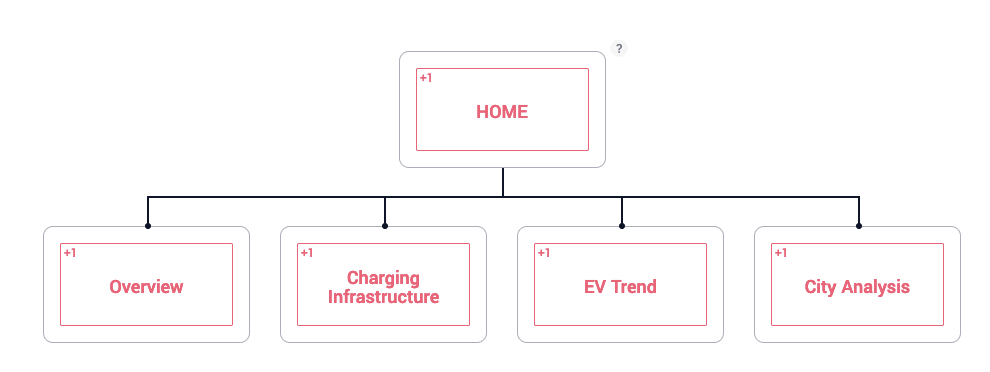
\includegraphics[scale=0.5]{Tree.png}
    \caption{Page Organization Tree}
    \label{fig:tree}
\end{figure}

%%%%%%%%%%%%%%%%%%%%%%%%%%%%%%%%%%%%%%%%%%%%%%%%%%%%
% HOME
%%%%%%%%%%%%%%%%%%%%%%%%%%%%%%%%%%%%%%%%%%%%%%%%%%%%
\subsection{Home Page}
Our home page shown in Figure \ref{fig:home} will contain a short
description of our data, our visualizations, and direct the user to the
information they are seeking.  Finally, the home page will let the user know the
purpose of our visualization.
\begin{figure}[ht]
    \centering
    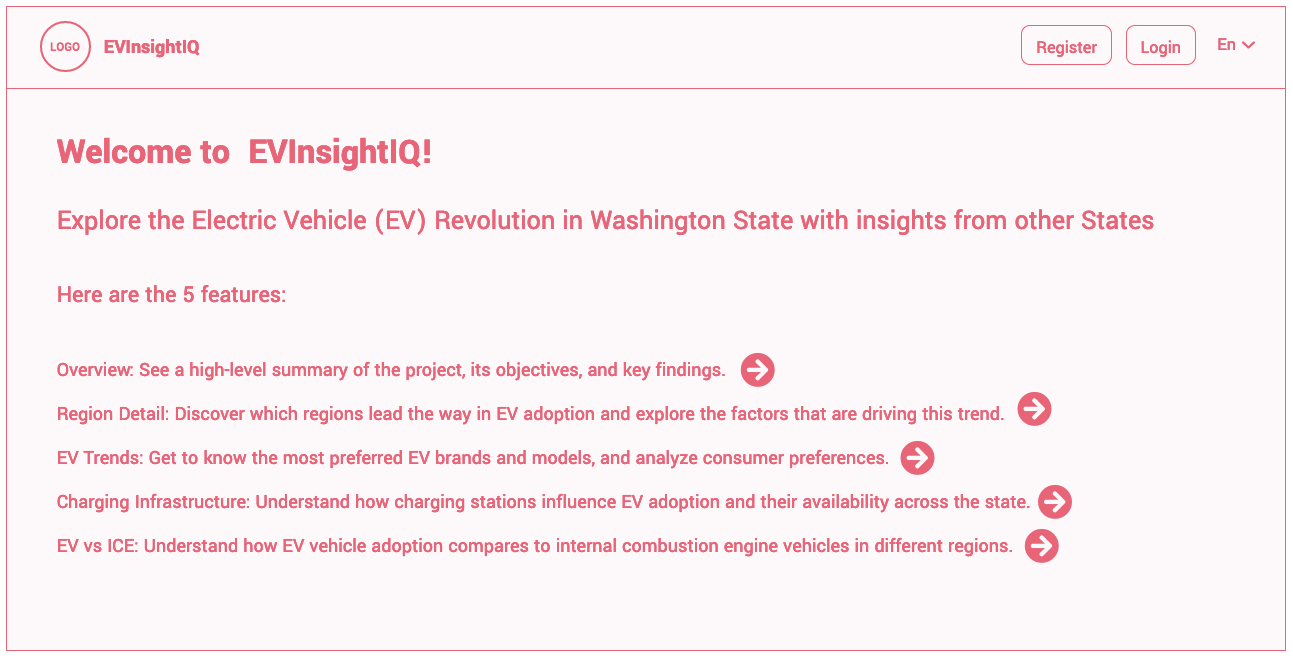
\includegraphics[scale=0.35]{Home}
    \caption{Home Page}
    \label{fig:home}
\end{figure}

\newpage
%%%%%%%%%%%%%%%%%%%%%%%%%%%%%%%%%%%%%%%%%%%%%%%%%%%%
% OVERVIEW
%%%%%%%%%%%%%%%%%%%%%%%%%%%%%%%%%%%%%%%%%%%%%%%%%%%%
\subsection{Overview}
The first visualization page will be our overview.  This page (Figure
\ref{fig:overview}) will give a broad understanding of the current number of
EV's registered, and charging stations, the overall growth trends for both. Also
it show the top EV brands and a map showing EV adoption rates by city.
\begin{figure}[ht]
    \centering
    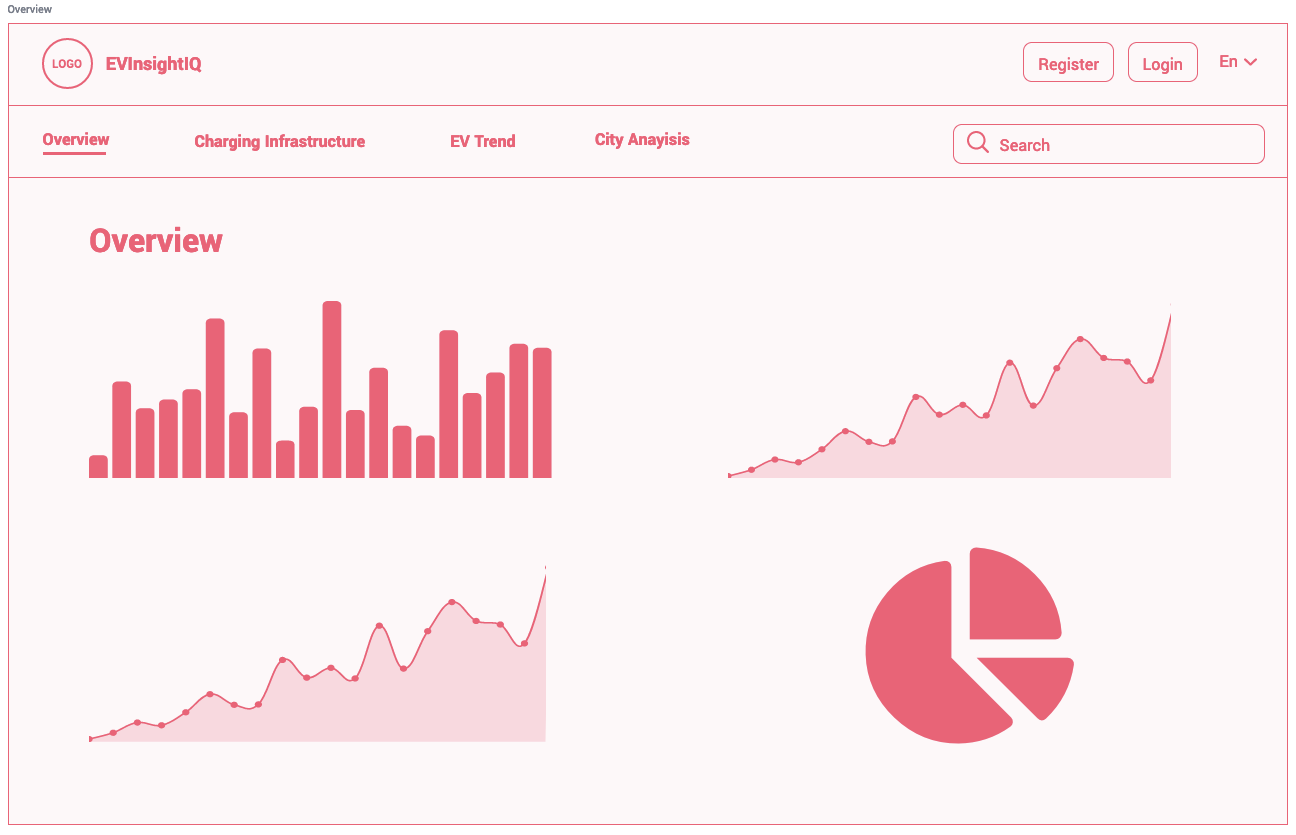
\includegraphics[scale=0.25]{Overview}
    \caption{Overview}
    \label{fig:overview}
\end{figure}

%%%%%%%%%%%%%%%%%%%%%%%%%%%%%%%%%%%%%%%%%%%%%%%%%%%%
% REGION DETAIL
%%%%%%%%%%%%%%%%%%%%%%%%%%%%%%%%%%%%%%%%%%%%%%%%%%%%
\subsection{Region Detail}
Next, will have a region details and analysis page (Figure \ref{fig:city}).
This page will contain comparison information between the State of Washington
and other states. Furthermore, one will be able to see a ranking of different
cities in Washington as well as other cities located in other states.  The user
will also be able to compare infrastructure growth and EV
adoption timelines with other cities and the mean adoption rates.
\begin{figure}[ht]
    \centering
    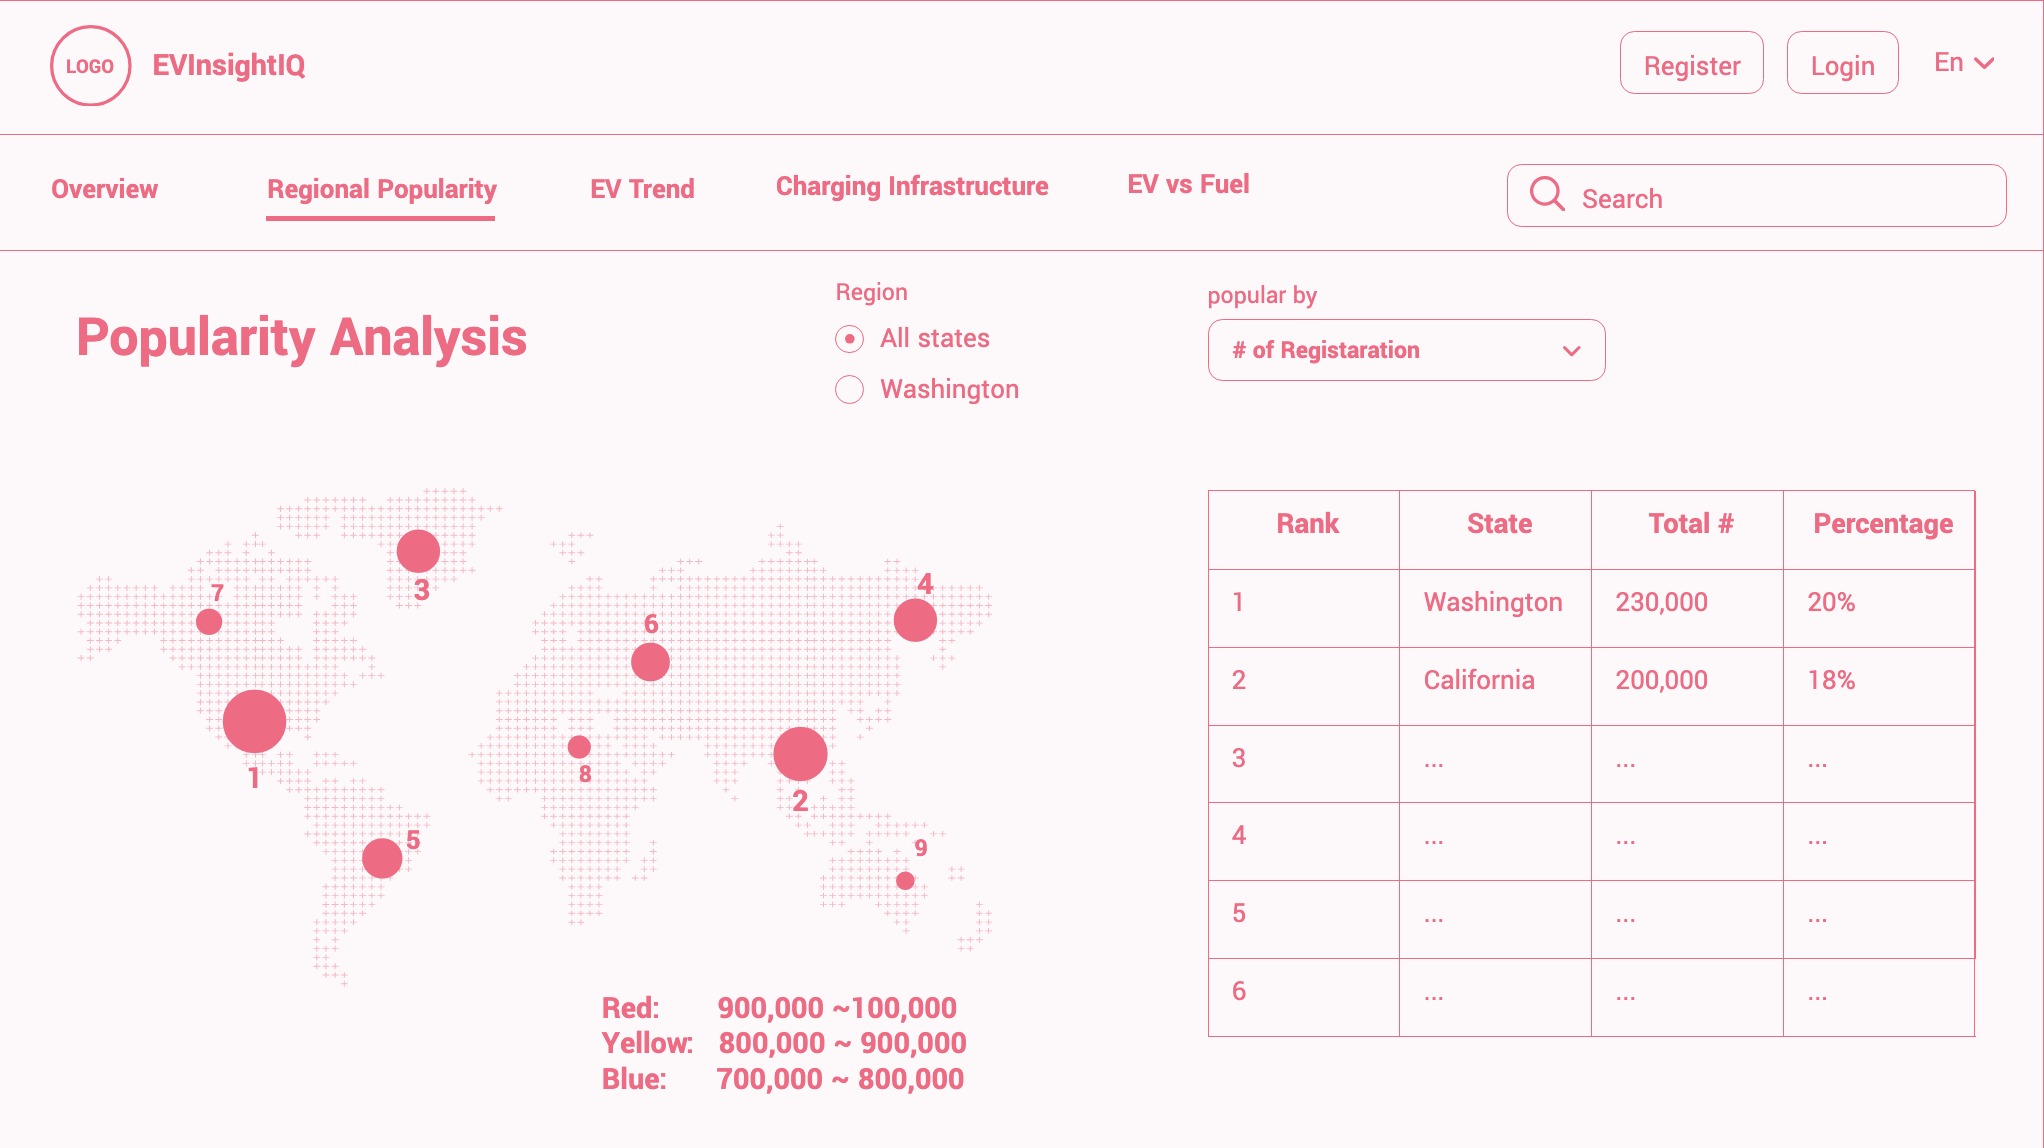
\includegraphics[scale=0.25]{Popularity Analysis}
    \caption{Region Detail}
    \label{fig:city}
\end{figure}

\newpage
%%%%%%%%%%%%%%%%%%%%%%%%%%%%%%%%%%%%%%%%%%%%%%%%%%%%
% EV TRENDS
%%%%%%%%%%%%%%%%%%%%%%%%%%%%%%%%%%%%%%%%%%%%%%%%%%%%
\subsection{EV Trends}
EV adoption trends will be shown on this page (Figure \ref{fig:evtrends}).
This page will show a comparison of car brands and models for certain time
frames.  Correlations between other state adoptions will be able to be
visualized with a timeline with laws and incentives highlighted or tool-tipped.
\begin{figure}[ht]
    \centering
    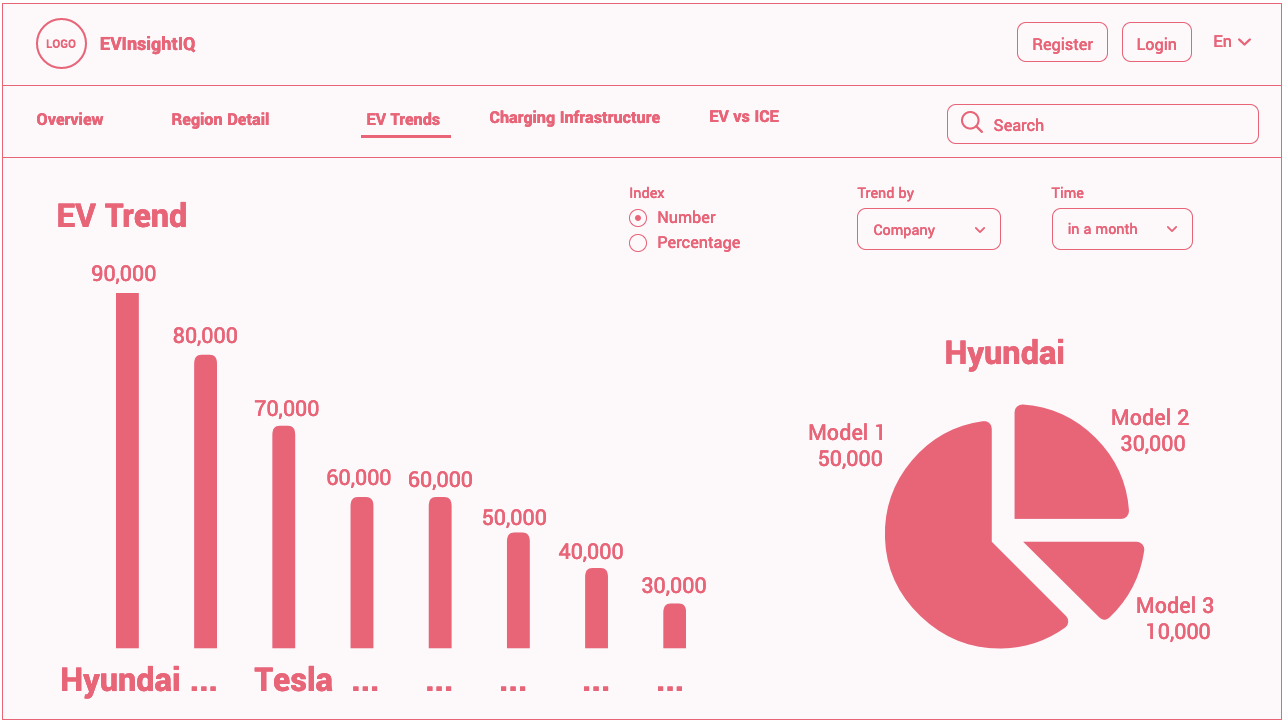
\includegraphics[scale=0.25]{EV Trends}
    \caption{EV Trends}
    \label{fig:evtrends}
\end{figure}

%%%%%%%%%%%%%%%%%%%%%%%%%%%%%%%%%%%%%%%%%%%%%%%%%%%%
% CHARGING INFRASTRUCTURE
%%%%%%%%%%%%%%%%%%%%%%%%%%%%%%%%%%%%%%%%%%%%%%%%%%%%
\subsection{Charging Infrastructure}
The third visualization page will provide a much deeper look into charging
infrastructure.  On this page (Figure \ref{fig:charge}), the user will be able
to compare the evolution of the charging infrastructure in Washington State and
other states in the US.  Similar to the EV Trends page, correlations between
different states will be able to be seen.  Finally, on a timeline graph, the
user will be able to see where legislation was put into effect so that the
results can be seen with respect to those laws and incentives.
\begin{figure}[ht]
    \centering
    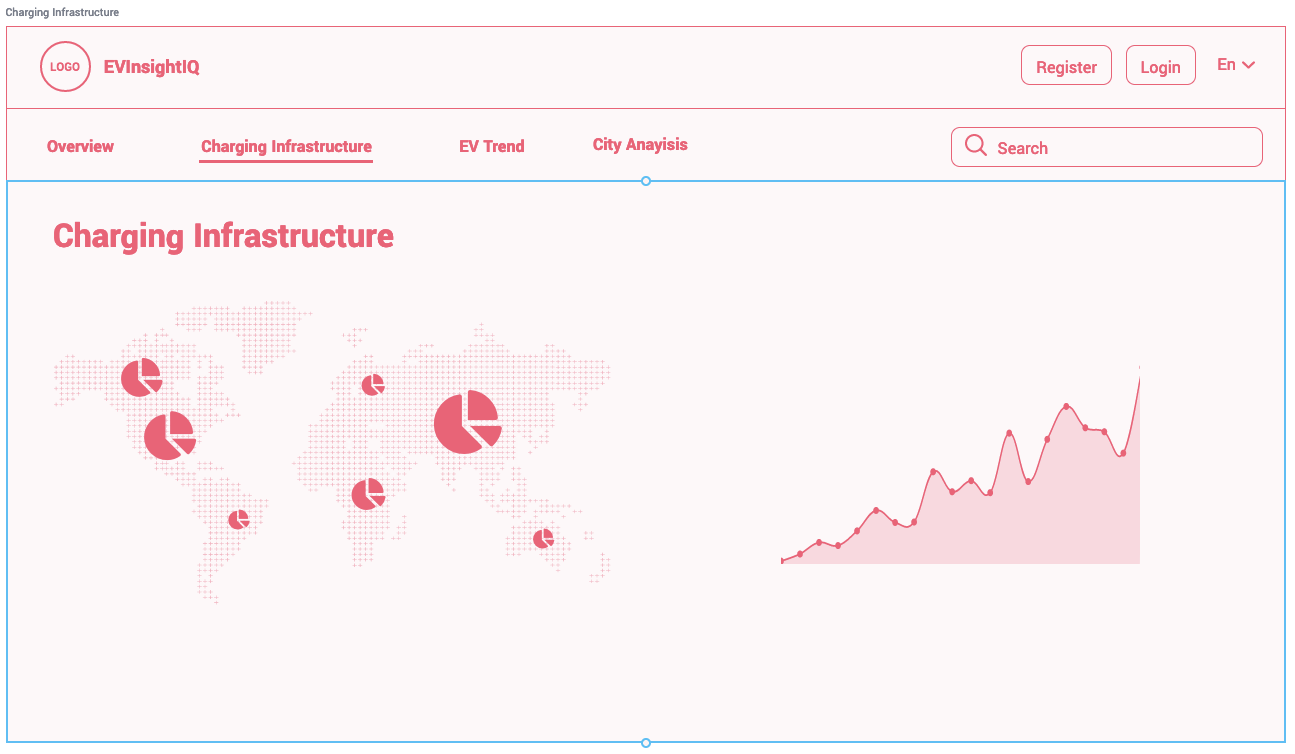
\includegraphics[scale=0.25]{Charging Infrastructure}
    \caption{Charging Infrastructure}
    \label{fig:charge}
\end{figure}

\newpage
%%%%%%%%%%%%%%%%%%%%%%%%%%%%%%%%%%%%%%%%%%%%%%%%%%%%
% EV vs ICE
%%%%%%%%%%%%%%%%%%%%%%%%%%%%%%%%%%%%%%%%%%%%%%%%%%%%
\subsection{EV vs Internal Combustion Engine (ICE) Vehicles}
Our final page will be a comparison of EV adoption against the landscape of
purchase trends of traditional internal combustion engine (ICE) vehicles (Figure
\ref{fig:evfuel}).  This data will be shown with respect to cities within
Washington State.  If we can hunt down and find out of state registration data,
we will attempt to include a comparison between different states as well.
\begin{figure}[!ht]
    \centering
    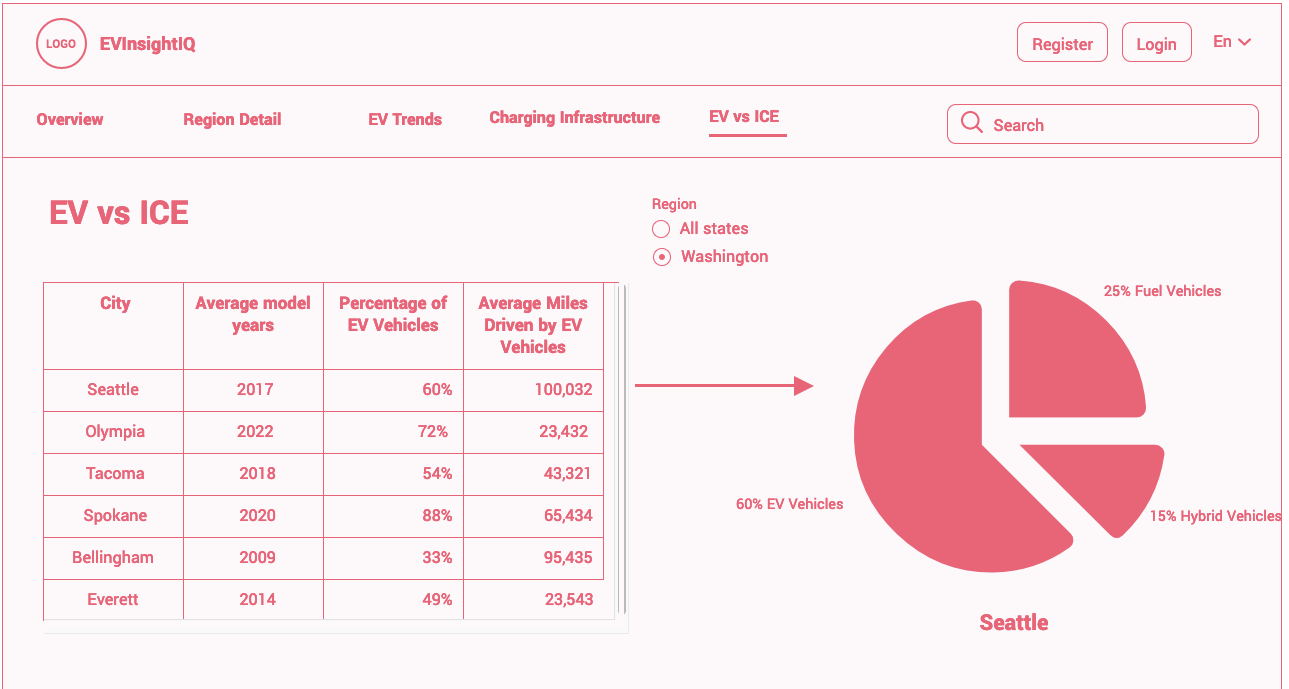
\includegraphics[scale=0.24]{EV vs Fuel}
    \caption{EV vs ICE}
    \label{fig:evfuel}
\end{figure}

\subsection{Access to wireframe}
\href{https://claritee.io/view/12733/14589/92384/1bf7a5d4-b9c8-42aa-a914-98842533efbf}{EV data visualization project}\\

\section{Data}
\subsection{Preprocessed and Cleaned}
\href{https://github.com/mk-imagine/csc805g5/tree/main/data}{GitHub Repository of Data}
\subsection{Source}
\href{https://data.wa.gov/Transportation/Electric-Vehicle-Population-Data/f6w7-q2d2}{Washington State Electric Vehicle Population Data}\vspace*{5pt}\\
\href{https://afdc.energy.gov/data_download}{Alternative Fuel Stations By State (Updated 10-12-2023)}\vspace*{5pt}\\
\href{https://afdc.energy.gov/data_download}{Washington State EV Laws and Incentives}\vspace*{5pt}\\
\href{https://www.atlasevhub.com/materials/state-ev-registration-data/}{EV
Registration Data By State} (This is a massive data set consisting of many data
sources.  Hence they will require further cleaning and integration -- this will
is an \emph{optional} set of data to be incorporated in our visualizations):
\begin{multicols}{4}
    \begin{enumerate}[topsep=0pt, partopsep=0pt, itemsep=1pt, parsep=1pt]
        % \setlength{\itemsep}{0pt}
        % \setlength{\parskip}{0pt}
        \item California
        \item Colorado
        \item Connecticut
        \item Florida
        \item Maine
        \item Minnesota
        \item Montana
        \item New Jersey
        \item New York
        \item North Carolina
        \item Oregon
        \item Tennessee
        \item Texas
        \item Vermont
        \item Virginia
        \item Wisconsin
    \end{enumerate}
\end{multicols}

\section{Technologies}
We plan to build the website using React, which offers a dynamic and interactive 
web-based environment. For data visualization, we will leverage Tableau, 
a powerful tool known for its effective data representation capabilities. 
To access the data, we will utilize tabular CSV files directly, which will
ensure simple and seamless data retrieval. Our project will be hosted statically
on GitHub. Using these technologies will allow us to leverage each of our team
members' strengths, while maintaining a realistic project scope.

\subsection{List of technologies to be used}
\begin{itemize}
    \item User Interface (UI): React
    \item Data Visualization: Tableau
    \item Data Source Handling: Incorporating CSV files within the project
    \item Hosting: GitHub for static website hosting
\end{itemize}
\end{document}